\subsection{Layer-Wise Relevance Decomposition}
\begin{figure*}
    \center
    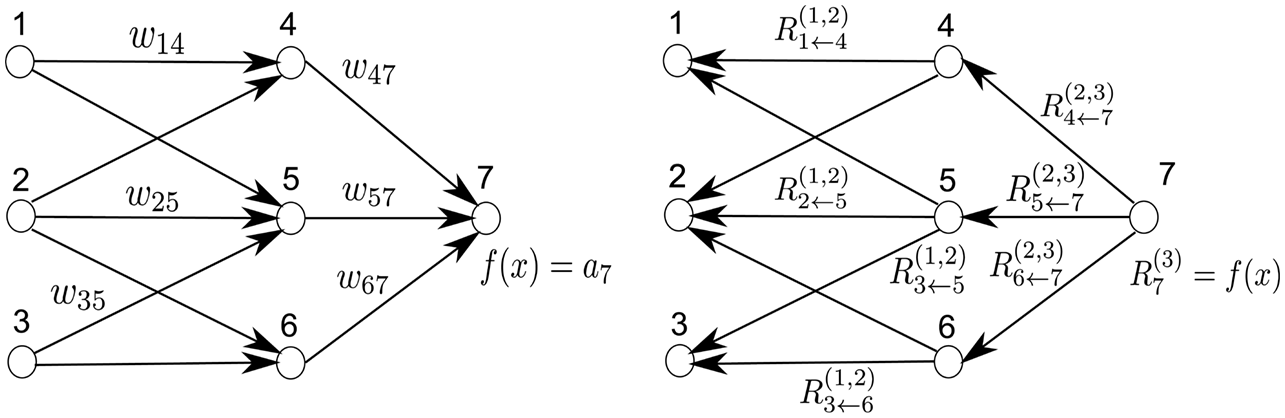
\includegraphics[]{lrp-fig2.PNG}
    \caption{\textbf{Left:} A neural network at prediction time. \textbf{Right:} a neural network at relevance-propagation time, adopted from \protect\cite{Bach.2015}}\label{fig:lrp-nn}
\end{figure*}
\gls{lrp} attempts to provide a measure for the \nameref{subsubsect:pixel-wise-decomp}, discussed earlier in \cref{subsubsect:pixel-wise-decomp}. The relevances are computed \textit{backwards} from the output of the model (\(f(x)\)) to its input (\(x\)) after prediction time. Relevance is denoted as \(R_{i}^{l}\), the relevance of neuron \(i\) in layer \(l\), where \(l=1\) is the input layer. \gls{lrp} is formulated by \fcite{Bach.2015} as a set of constraints:
\begin{enumerate}
    \item \gls{lrp} must follow \ref{subsubsect:pixel-wise-decomp} completely.\label[const]{enum:gls-1}
    \item each layer of the neural network can be represented by relevances, such that 
    \begin{multline}
        f(x) = \dots \\ 
        = \sum_{j\in l+1} R_j^{(l+1)} = \sum_{i\in l} R_i^{(l)} \\
        = \dots = \sum_{h\in x} R_h^{(1)}.\label{eq:lw-propagation}
    \end{multline}
    Informally, \cref{eq:lw-propagation} implies that relevances can be propagated from the predictor-output \(f(x)\) to the input-variables in \(x\).\label[const]{enum:gls-2}
    \item the relevance of the \textit{output neuron} is defined as the model-output \(f(x)\).\label[const]{enum:gls-3}
    \item the relevance of \textit{every other neuron} is the sum of its incoming \glspl{message}, formally 
    \begin{equation}
        R_i^{(l)} = \sum_{\left\{ j | \text{Path } P_{i \rightarrow j} \text{ exists}\right\}} R_{i\leftarrow j}^{(l, l+1)}.\label[constraint]{eq:incoming-messages}
    \end{equation}\label[const]{enum:gls-4}
    \item the total relevance that a neuron sends out as \glspl{message} is equal to its own relevance, formally
    \begin{equation}
        R_j^{(l+1)} = \sum_{\left\{ i | \text{Path } P_{i \rightarrow j} \text{ exists}\right\}} R_{i\leftarrow j}^{(l, l+1)}.
    \end{equation}\label[const]{enum:gls-5}
    \item each \gls{message} \(R_{i\leftarrow j}^{(l,l+1)}\) is the product of the relevance of neuron \(j\), \(R_j^{(l+1)}\), weighted by the \textit{relative strength} of the path \(P_{i\rightarrow j}\), formally
    \begin{equation}
        R_{i\leftarrow j}^{(l,l+1)} = R_{j}^{(l+1)} \frac{a_i w_{ij}}{\sum_{h\in (l)} a_h w_{hj} + b_j},\label{eq:weighted-message}
    \end{equation}
    where \(a_i\) is the output of neuron \(i\) (precisely the output of its activation-function), \(w_ij\) are the weights that connect neurons \(i \text{ and } j\) and \(b_j\) is the bias for layer \(j\). 
    \par
    \Cref{eq:weighted-message} shows the simplest case of a \textit{weighting}-term. Different approaches for stabilizing the propagation, such as \(\alpha\beta\)-\gls{lrp} and \(\epsilon\)-\gls{lrp}, are further discussed in~\cite[20-22]{Bach.2015}.\label[const]{enum:gls-6}
\end{enumerate}
In summary, \gls{lrp} requires a conservation of relevance between layers (\cref{enum:gls-2}), the relevance of a neuron to be both the sum of its incoming weighted \glspl{message} (\cref{enum:gls-4,enum:gls-6}) and the sum of its outgoing weighted \glspl{message} (\cref{enum:gls-5,enum:gls-6}).

\subsection{Taylor-Decomposition}
As an approximation to \gls{lrp}, Taylor-Decomposition was proposed in~\cite{Bach.2015}. It directly defines relevances \(R_{h}^{(1)}\) at the (slightly modified) input-sample \(x'\) and therefore avoids the process of decomposing relevances for each layer. Instead, relevance \(R_{h}^{(1)}\) is defined by developing a first order Taylor series of the input \(x\) around a root point \(x_0\), such that \(f(x_0) = 0\). Informally, Taylor-Decomposition attributes relevance by weighting the difference of the image and the root point (\(x-x_0\)) with the partial derivative of the predictor with respect to the input \(x\). Formally
\begin{equation}
    R_{h}^{(1)} \approx (x-x_0)_{(h)} * \frac{\partial f}{\partial x_{(h)}}(x_0).
\end{equation}
Here, \(x'\) as mentioned above is \(x':=x-x_0\).
\par
Again, a set of constraints is formulated to find the root-point \(x_0\)
\begin{enumerate}
    \item \(x_0\) must be a root point of \(f\), such that \(f(x_0)=0\)
    \item \(x_0\) must be in the neighborhood of \(x\) under some distance metric, e.g.\ the Euclidean L2-norm.\label[const]{enum:taylor-closeness}
\end{enumerate}
A major issue with Taylor-Decomposition is satisfying \cref{enum:taylor-closeness}. \fcite{Bach.2015} do not provide a solution for sparsely populated data-domains, e.g.\ datasets of natural images. Yet, when the root point is ill-defined, \fcite{Kindermans.2019} were able to show that Taylor-Decomposition produces bad results.

\subsection{Deep-Taylor-Decomposition}
Deep-Taylor-Decomposition as proposed by \fcite{Montavon.2017} tries to overcome the difficulties that the search for root-points according to \cref{enum:taylor-closeness} posed to simple Taylor-Decomposition. For this, they introduce axioms \ref{ax:positivity} and \ref{ax:consistency} which Deep-Taylor-Decomposition must satisfy. Also, they propose a method for finding root-points \(x_0(i):= x_i + t*v_i\), where \(v_i\) is called \textit{search direction}. \citeauthor{Montavon.2017} use this definition to define a set of weighting terms, similar to those in \gls{lrp} and Taylor-Decomposition. Formally, they introduce a generalization of the weighting parameter in \cref{eq:weighting-in-dtd}\cite[see][Supplementary Material]{Montavon.2017}
\begin{equation}
    R_{i\leftarrow j}^{(l,l+1)} = \sum_j \frac{v_i w_{ij}}{\sum_i v_i w_{ij}} R_j^{(l+1)}\label{eq:weighting-in-dtd}
\end{equation}
and then derive specific weighting parameters by defining \(v_i\).
\begin{description}
    \item[\(\symbfit{w^2}\)-Weighting] which is similar to \cref{eq:weighted-message} but does only rely on the weights \(w_{ij}\) that connect \(i \text{ and } j\). \(v_i\) is chosen to be \(v_i:=w_{ij}\).
    \begin{equation}
        R_{i\leftarrow j}^{(l,l+1)} = R_{j}^{(l+1)} \frac{w_{ij}^2}{\sum_{h\in (l)} w_{hj}^2}.\label{eq:w2-weighting-dtd}
    \end{equation}
    \(w^2\)-Weighting is used, when the input-domain is unrestricted, i.e.\ \(x\in \mathbb R^{|x|}\).
    \item[\(\symbfit{z^+}\)-Weighting] is similar to the \(\alpha \beta\)-Rule of \gls{lrp}, with \(\beta=0, \alpha=1\). Here, \(v_i\) is the set of all \(x_i\) for which the correspoding \(w_{ij}\) is positive, formally \(w_{ij}^{+} = \left\{w_{ij} | w_{ij}\geq 0\right\}\) and \(v_i:=\left\{x_i|w_{ij}\in w_{ij}^{+}\right\}\). The weighting therefore is
    \begin{align}
        R_{i\leftarrow j}^{(l,l+1)} &= R_{j}^{(l+1)} \frac{x_i w_{ij}^{+}}{\sum_{h\in (l)} x_(h) w_{hj}^{+}}\\
        R_{i\leftarrow j}^{(l,l+1)} &= R_{j}^{(l+1)} \frac{z{ij}^{+}}{\sum_{h\in (l)} z_{hj}^{+}},
    \end{align}
    with \(z_{ij}^{+}:= x_i w_{ij}^{+}\), from which the name \(z^{+}\)-Weighting is derived.
    \(w^2\)-Weighting is used, when the input-domain is unrestricted, i.e.\ \(x\in \mathbb R^{|x|}\).
    \item[\(\symbfit{z^{\mathscr B}}\)-Weighting] placeholder 
\end{description}
\par
\blindtext[1]
\paragraph{Relevance-Models}
\blindtext[1]